\documentclass[11pt,a4paper]{article}

\usepackage[margin=1in]{geometry}
\usepackage{amsmath,amssymb,amsthm}
\usepackage{graphicx}
\usepackage{booktabs}
\usepackage{siunitx}
\usepackage{hyperref}
\usepackage{xcolor}
\usepackage[numbers,sort&compress]{natbib}
\usepackage{tikz}
\usetikzlibrary{arrows.meta,positioning}
\usepackage{caption}
\usepackage{array}

\hypersetup{colorlinks=true,linkcolor=blue!50!black,citecolor=blue!50!black,urlcolor=blue!50!black}
\sisetup{detect-all,per-mode=symbol}
\newcommand{\hyp}[1]{\textcolor{blue!45!black}{\textsf{\small #1}}}

\title{\textbf{A Compact \SI{7}{\mega\electronvolt} SSMB-Compton Architecture\\
for a Coherent \SI{13.5}{\nano\meter} Lithography Source}\\[4pt]
\large Architecture~II of the lumen EUV source family (rank~3); shared experimental gate with the
storage-ring SSMB undulator architecture}

\author{lumen verified-hypothesis lab \\ \texttt{dancinlab/lumen}}
\date{Draft, as-of 2026-06}

\begin{document}
\maketitle

\begin{abstract}
We specify a \emph{metre-scale} EUV source architecture that combines steady-state microbunching
(SSMB) with laser-Compton up-conversion. Inverse-Compton scattering reaches \SI{13.5}{\nano\meter}
from a \SI{7}{\mega\electronvolt} electron beam ($\sim\!455\times$ less energy than the undulator
route), at a $\sim$\SI{2.3}{\centi\meter} bending radius that yields a $\sim$\SI{1}{\meter} tabletop
ring; and because Compton up-conversion has no free-electron-laser gain condition, the source is
\emph{slice-energy-spread immune}. Adding SSMB makes it coherent and continuous-wave. The result is a
compact, coherent, CW, slice-immune EUV source --- the tabletop ambition reached by a different
mechanism than the slice-spread-bound single-pass FEL. The binding residual is a Compton
bandwidth-collection flux tax ($\sim\!50\times$), recoverable only by stacking an IR enhancement
cavity and energy-recovery current at their demonstrated maxima simultaneously. The architecture
shares its single experimental gate --- steady-state microbunching at \SI{13.5}{\nano\meter}
precision --- with the storage-ring SSMB undulator architecture (companion paper~I): one experiment
de-risks both. The analysis is closed-form and reference-matched; it claims convergence on the same
physics, not precedence.
\end{abstract}

\section{Introduction}
This is Architecture~II of the lumen EUV source family (rank~3). It is the second of two \emph{novel}
architectures; the first (rank~2, paper~I) is the storage-ring SSMB undulator. The two are genuinely
different machines --- here \SI{7}{\mega\electronvolt} and inverse-Compton, there
$\sim$\SI{511}{\mega\electronvolt} and an undulator --- so we document them separately, while making
explicit that they reduce to one shared experimental gate (Section~\ref{sec:gate}). This architecture
is the more aggressive: it targets a true tabletop footprint.

\section{Background: sidestepping the slice-spread wall}
For an undulator FEL, gain collapses once $\sigma_\delta/\rho\gtrsim1$~\citep{mingxie}; a
\SI{0.5}{\percent} laser-plasma beam never lases at \SI{13.5}{\nano\meter} (\hyp{H\_031}; demonstrated
LPA-FEL floor $\sim$\SI{25}{\nano\meter}~\citep{xiao2026}). Inverse-Compton scattering of a drive
laser ($\lambda_x\approx\lambda_L/4\gamma^{2}$) has \emph{no} Pierce gain condition: slice spread only
broadens the line, so the architecture reaches \SI{13.5}{\nano\meter} at very low beam energy
(\hyp{H\_033}). This is the mechanism the single-pass LPA-FEL (rank~6) cannot use and why that path is
terminal-thin (\hyp{H\_038}).

\section{Architecture}
\label{sec:arch}
\begin{figure}[t]
\centering
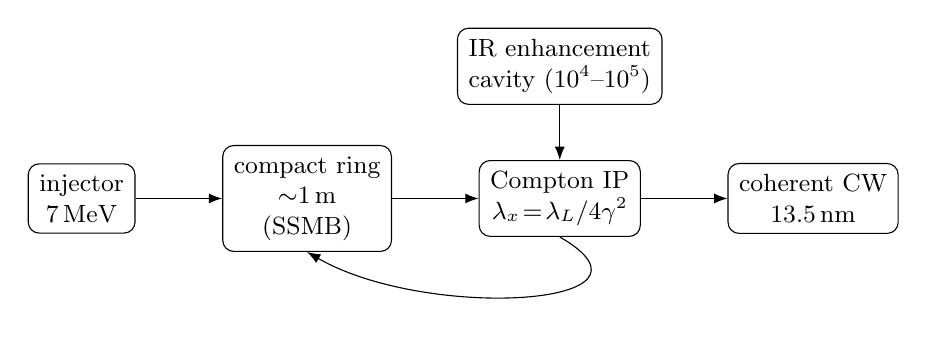
\begin{tikzpicture}[node distance=7mm and 11mm,every node/.style={font=\small},
  box/.style={draw,rounded corners,align=center,inner sep=4pt,minimum height=8mm}]
  \node[box] (gun) {injector\\\SI{7}{\mega\electronvolt}};
  \node[box,right=of gun] (ring) {compact ring\\$\sim$\SI{1}{\meter}\\(SSMB)};
  \node[box,right=of ring] (ip) {Compton IP\\$\lambda_x\!=\!\lambda_L/4\gamma^2$};
  \node[box,above=of ip] (cav) {IR enhancement\\cavity ($10^{4}$--$10^{5}$)};
  \node[box,right=of ip] (out) {coherent CW\\\SI{13.5}{\nano\meter}};
  \draw[-{Latex}] (gun)--(ring); \draw[-{Latex}] (ring)--(ip); \draw[-{Latex}] (ip)--(out);
  \draw[-{Latex}] (cav)--(ip);
  \draw[-{Latex}] (ip.south) to[out=-30,in=-30,looseness=1.4] (ring.south);
\end{tikzpicture}
\caption{Compact SSMB-Compton architecture. A \SI{7}{\mega\electronvolt} microbunched beam in a
$\sim$\SI{1}{\meter} ring scatters an IR drive laser (recirculated in an enhancement cavity) at the
interaction point; Compton up-conversion to \SI{13.5}{\nano\meter} is slice-spread immune.}
\label{fig:arch}
\end{figure}

At \SI{7}{\mega\electronvolt} the bending radius is $\sim$\SI{2.3}{\centi\meter} (\SI{1}{\tesla}),
giving a metre-scale ring (\hyp{H\_044}). Combining SSMB microbunching (coherent CW) with Compton
up-conversion at low energy yields a compact + coherent + CW + slice-immune source. The residual is a
\textbf{flux tax}: the small Thomson cross-section puts the demonstrated Compton flux
($\sim\!10^{13}$~ph/s) $\sim\!7\times10^{5}$ below the $\sim\!6.8\times10^{18}$~ph/s needed for
\SI{100}{\watt} (\hyp{H\_034}). Recirculation closes most of it: an IR-wavelength enhancement cavity
(finesse $10^{4}$--$10^{5}$ --- an EUV cavity is forbidden by multilayer $R\!\approx\!0.70$,
\hyp{H\_035}) times energy-recovery average-current gain ($\sim\!10^{3}$) gives $\sim\!10^{7}$,
exceeding the gap. But bandwidth-limited collection (a \SI{2}{\percent} in-band passband from the
wide low-$\gamma$ cone) derates flux $\sim\!50\times$ (\hyp{H\_036}); it is recovered only by running
finesse and current at their demonstrated maxima \emph{simultaneously}. A brightness lever does not
help --- the $\lambda$--$\theta$ correlation is radiation kinematics, beam-independent (\hyp{H\_037},
a recorded negative). A 2025 cavity-based compact EUV-litho proposal occupies this space
\citep{he2025}.

\paragraph{Subsystems and secondary gates.} Beyond the shared microbunching gate: the joint
finesse$\times$current maximum at EUV, the IR drive cavity integration, and Compton flux extraction.

\section{The shared gate}
\label{sec:gate}
The architecture rests on one unproven step: steady-state microbunching at \SI{13.5}{\nano\meter}
precision ($\sigma_z\!\approx\!\SI{3}{\nano\meter}$), physics-allowed with coherent fraction
$b^2\approx0.14$ ($b=\exp(-\tfrac{1}{2}(2\pi\sigma_z/\lambda)^2)$) (\hyp{H\_046}). \textbf{The same
gate binds the storage-ring SSMB undulator architecture (paper~I), so one experiment de-risks both}
(\hyp{H\_048}). The route trade is exactly one axis: this architecture is metre-scale but pays the
$\sim\!50\times$ Compton tax that the undulator route avoids at the cost of a larger ring. The
cooling lever the lab derived closed-form (\hyp{H\_024}) is what the latest SSMB frontier adds (OSC,
\citep{deng2025}; \hyp{H\_050}).

\section{Related work and limitations}
The SSMB mechanism was demonstrated by \citet{deng2021}; compact inverse-Compton sources are
operational at hard X-ray and $\gamma$ energies; a compact cavity-based EUV-litho source is proposed
in \citet{he2025}. All relations are first-order, closed-form, representative-parameter. The Compton
flux tax is the binding gate after microbunching; \SI{13.5}{\nano\meter} power from a compact
SSMB-Compton ring is undemonstrated (concept stage). This is reference-match, not priority.

\section{Reproducibility and future work}
Closed-form evidence: lumen \texttt{HYPOTHESES/cards/H\_\{033,034,035,036,037,044,046,048,050\}.md} +
deterministic runners in \texttt{state/h0*/}; re-verify with \texttt{python3 tool/qa.py}. Decisive
next step: demonstrate steady-state microbunching at \SI{13.5}{\nano\meter} ($b^2\gtrsim0.1$ over
$\gtrsim\!10^{3}$ turns), then the Compton flux-tax recovery at the joint operating point. If
$\sigma_z\gtrsim\!\SI{10}{\nano\meter}$ or the derate exceeds the recoverable margin, the concept
reverts to longer wavelengths (where $b^2\!\to\!1$).

\bibliographystyle{unsrtnat}
\bibliography{references}
\end{document}
